\documentclass[11pt]{article}
\usepackage{url}
\usepackage{color}
\usepackage[pdftex]{graphicx}
\usepackage{amsmath}
\usepackage{fancyhdr}
\usepackage[margin=1in,footskip=0.25in]{geometry}
\usepackage{hyperref}

\pagestyle{fancy}
%\pagestyle{empty}

\title{Tfit Notes}
\author{Robin D. Dowell}
\date{}
\lhead{Tfit Design Notes}
\rhead{Dowell}
\date{ }

\begin{document}
\maketitle
\noindent $*$ Corresponding author: robin.dowell@colorado.edu

This document assumes that the github Tfit tree has been checked out into a 
directory called "Tfit".   Within the Tfit code base the primary code for the 
algorithm lives in Tfit/src and is written in C++.   Compiling the code is 
done via the Makefile system (cd Tfit/src/; make). 

\section{Coding conventions}
Unit tests use the gmock/gtest framework from Google.
Testing uses cMake to build the appropriate tests (cd Tfit/test/build; cmake .. ; make; ./TestTfit).  
General naming convention for tests is for every .cpp file within 
Tfit/test/src we have a test file of the same name prefaced by test\_.  For
example, Tfit/src/filename.cpp has a corresponding Tfit/test/src/test\_filename.cpp

Within this test file, individual objects are the test set name and test 
names follow the method\_behavior naming 
convention.  Note that for gtest: Test(test set name, test name).  Fixture
classes (TEST\_F) are used when the setup of a test needs to be 
repeated frequently.  In these cases the class name is infoNameTest where
infoName is some informative name that includes the Class name.
All methods/classes with logic (i.e. getters and setters generally do not 
have logic, unless they test the inputs) should have a Unit test.

Test coverage statistics and reports can be obtained through gcov
and lcov using the same Makefile (cd Tfit/test/build; cmake ..; make;
./TestTfit; make gcov; make lcov).  Note that lcov produces web parsable
coverage reports (file:///.../Tfit/test/build/lcoverage/index.html).

Furthermore, the code (both main code base Tfit/src and Unit testing 
    Tfit/test/src) have documentation following Doyxgen standards.   
The Doxygen configuration file
lives at Tfit/docs/doxyfile.in and documentation can be built (cd Tfit/docs; 
    doxygen doxyfile.in).   This manual resides within Tfit/docs/manual and 
is built using a Makefile (cd Tfit/docs/manual; make all ).  UML diagrams are
constructed using metapost (*.mp).  A User's guide has been stubbed and should
eventually be makeable via make userguide.

\section{Big Picture Stuff}
Some rough initial thoughts on which programs are available:

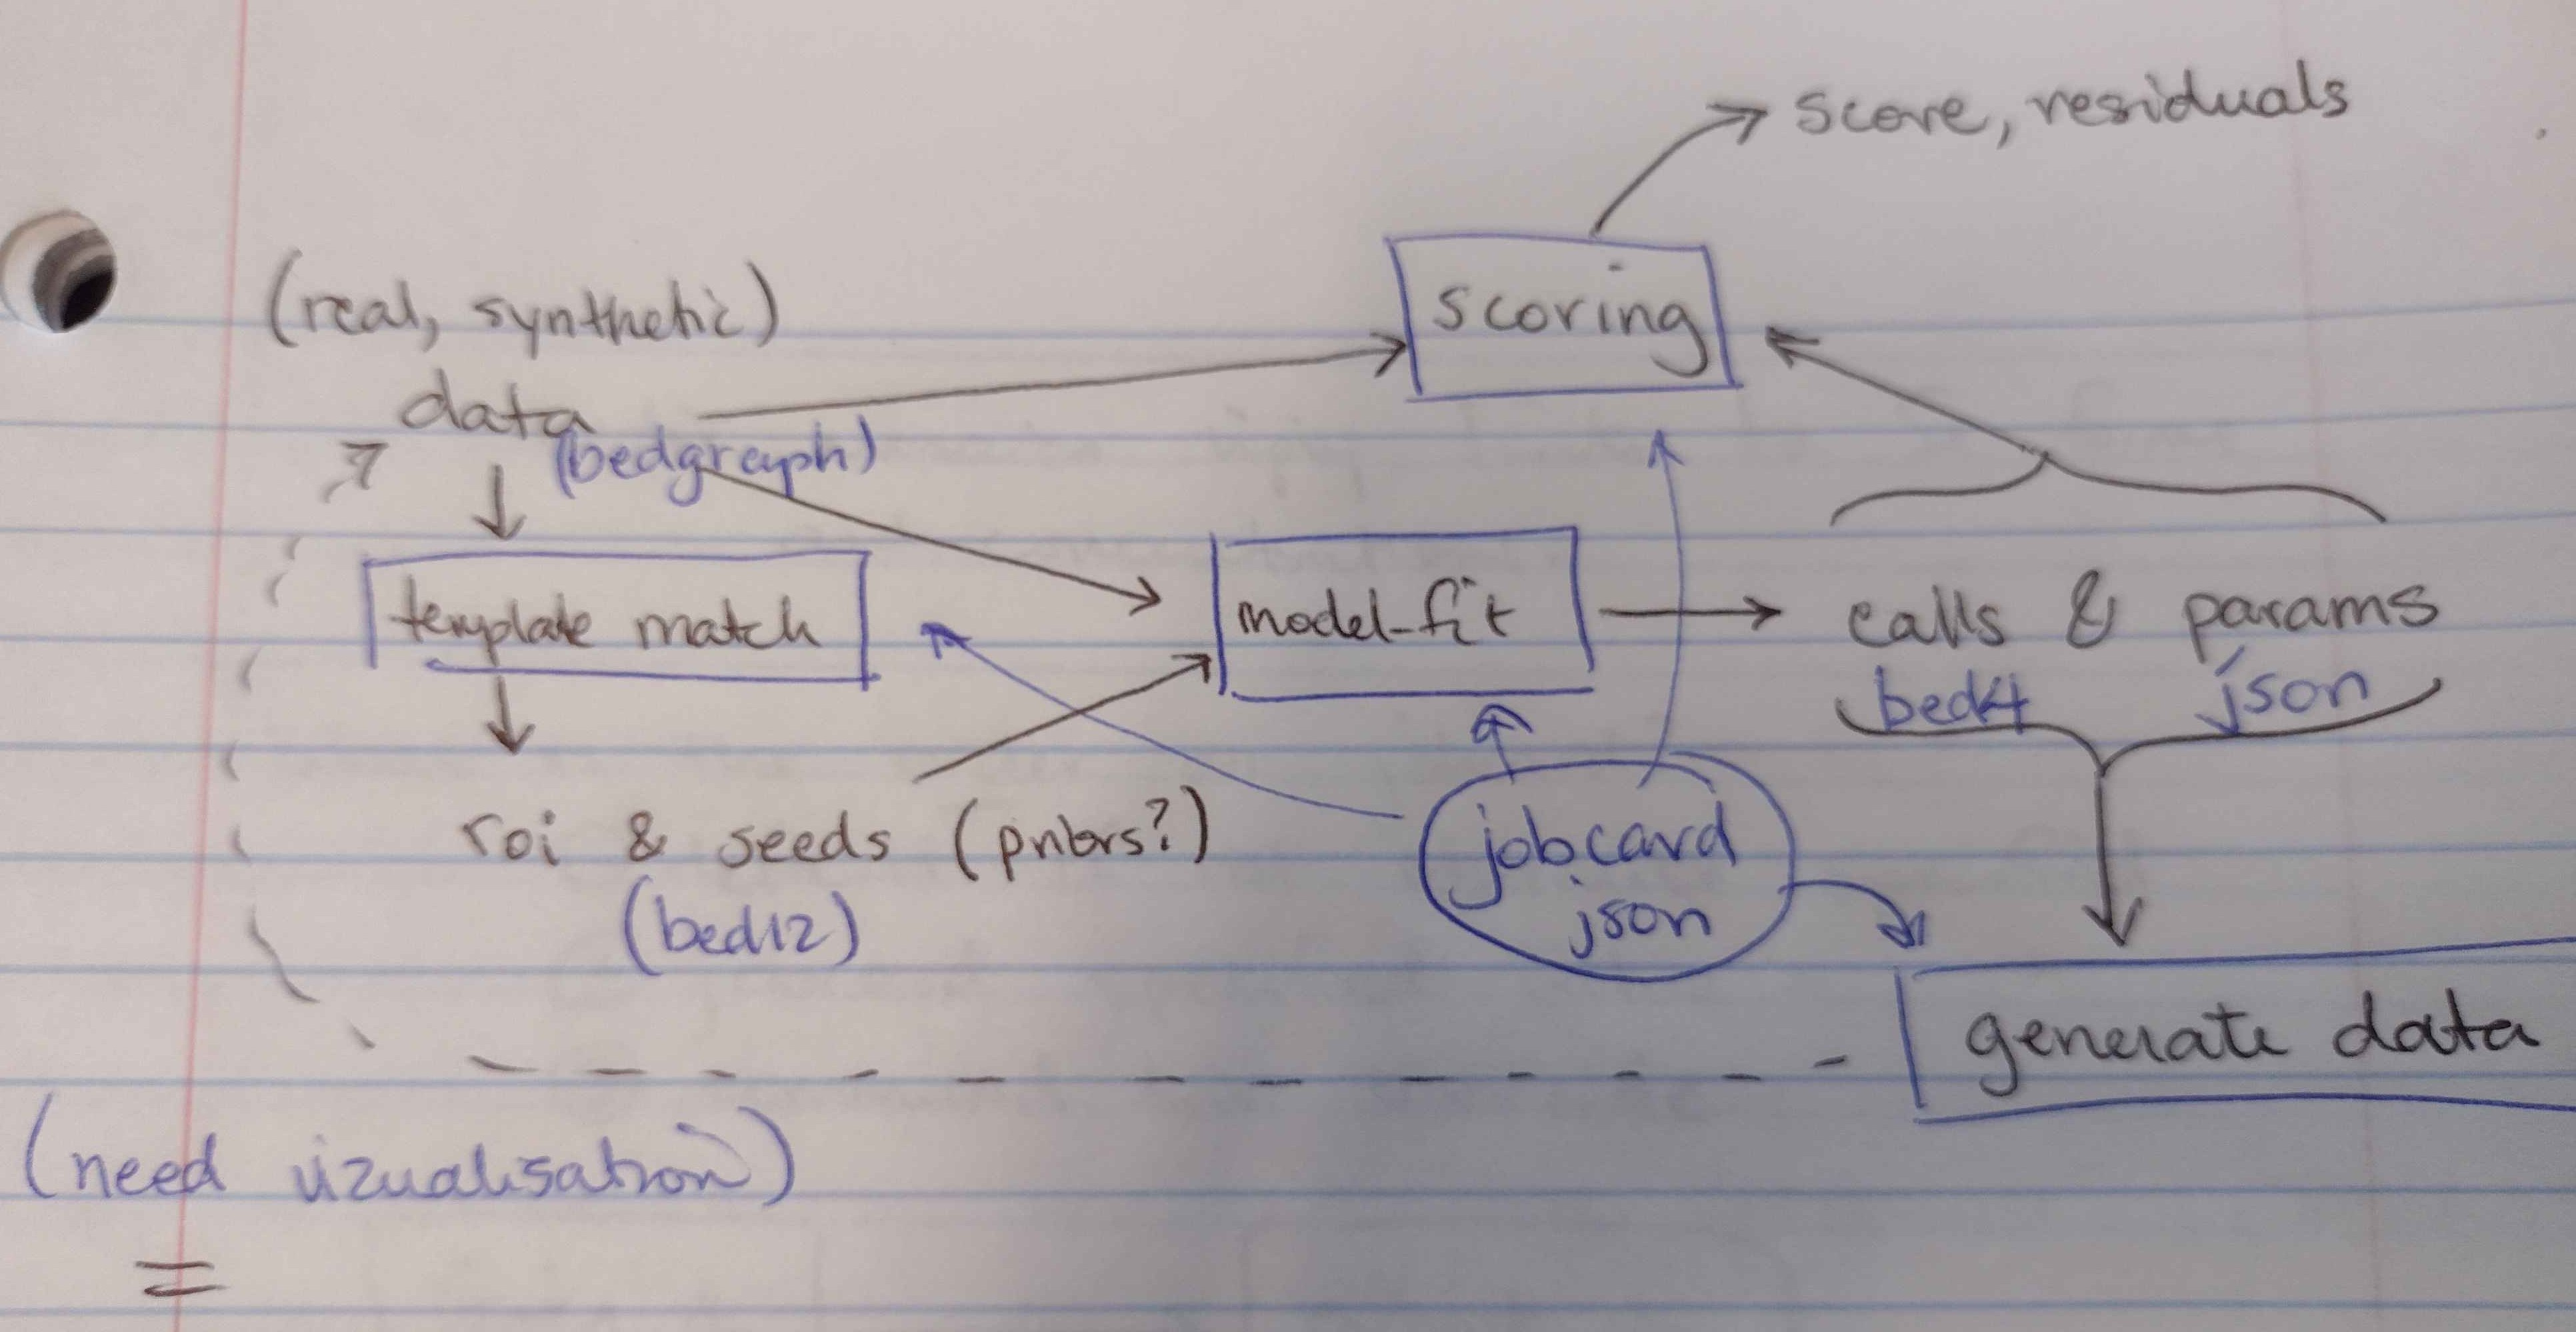
\includegraphics[width=\textwidth]{figs/ProgramsNotes.jpg}

\textbf{Expect:} 
\begin{enumerate}
\item Fit model to data by reading bedGraph (dInterval) -- this either
  produces a bed12 (if only bedGraph) or is only read within ROI (if bed given).  
  This is then used to fit model producing model\_fits for each gInterval.
\item Generate data by reading in model\_fits from which data is generated
    into a dInterval which is then converted into a gInterval for reporting.
\item Scoring involves reading in both a dInterval (bedGraph) and a model\_fit
  from which we can score the data and calculate residuals.
\item Template matching reads in the bedGraph and from this calculates seeds.
\end{enumerate}

Some rough initial thoughts on the convention/hierarchy in running a program:

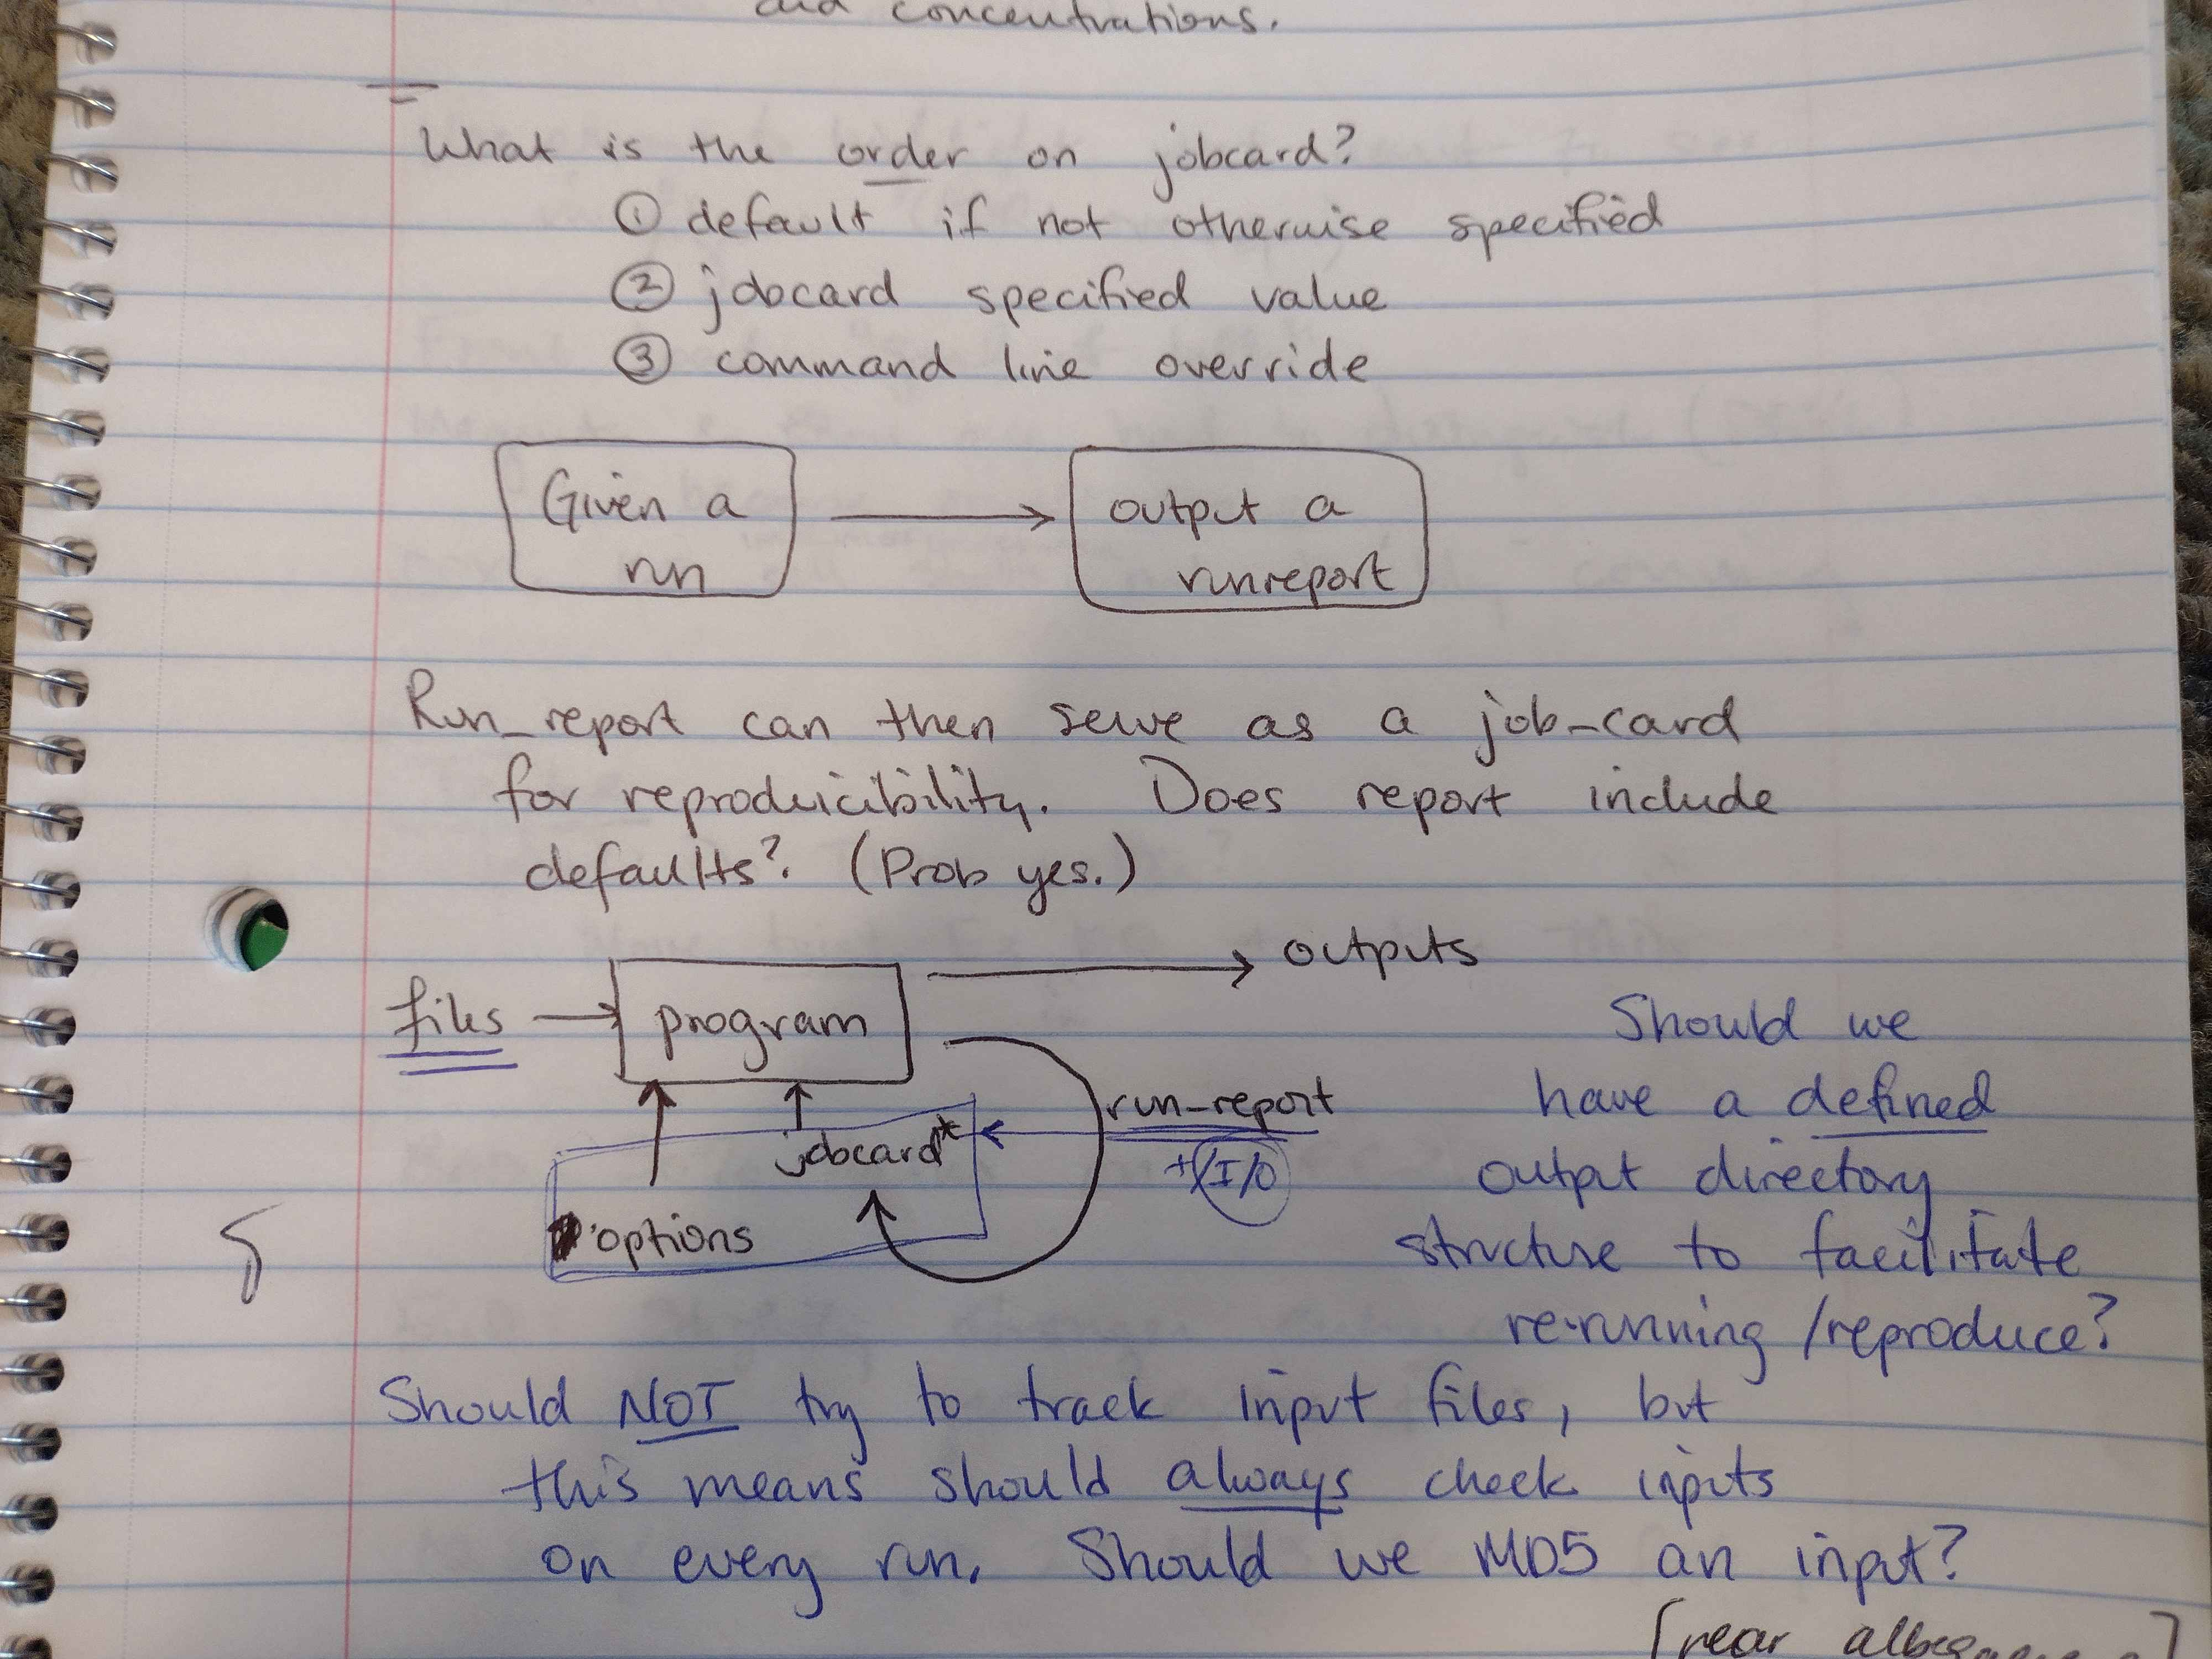
\includegraphics[width=0.7\textwidth]{figs/RunNotes.jpg}

\section{Data Handling Design}
Tfit uses signed bedGraphs as data input.  A bedGraph has the basic format of: 
chromosome start stop coverage (tab delimited).  Tfit assumes all coordinates are
reported as zero based half open coordinates, as described in the bedGraph 
standard.  

The coverage value is expected to be signed according to strand (e.g. positive 
numbers refer to the positive strand whereas negative numbers refer to the 
negative strand).  Thus each position in the genome may be represented in a 
signed bedGraph twice, once per sign/strand.

%\includegraphics{datahandling1.mps}  OLD DESIGN
\includegraphics{datahandling21.mps}

\textbf{March 2023:} The Model design was altered to create a container 
(now called gInterval) that holds the RawData, dInterval and bed12 contents. 
With this change, the RawData no longer is an intermediary between the dInterval
and the old gInterval (now renamed bed4).  

Tfit attempts to fit one or more instances of the RNA polymerase model to a 
region of interest.  If the only input is the signed bedGraph, the regions of 
interest are inferred directly from the bedGraph (chromosome identifiers 
and coordinates). In this scenario the bedGraph is read into RawData which 
builds the bed12 segments.

Alternatively (and the preferred method), the user can provide a bed 
file (bed3, bed4, bed6, or bed12) to specify the regions of interest.  Each 
line of a bed file is stored as the corresponding portion of the bed12 object.
When a user provides a ROI bed file, Tfit will *only* consider data within 
these regions (e.g. bed12 correspond to bed entries and data outside these 
regions is ignored).  In this scenario the bed is read into the bed12 and for 
each bed12 the bedGraph is read via the PointCov/RawData. 

Generally, bedGraphs are read in as PointCov (position, coverage) in a strand 
specific fashion within the RawData object.  Notably, the bed12 format is 
adapted here to provide Tfit with seed information.  [See the Seeds object and 
information (Section \ref{seeds}) for more details.] Seeds: It is worth noting 
that bed12 data is interpreted in a very specific way in the Tfit framework.   
Exon lengths are weights and exon starts are positions for possible seeds 
to the EM algorithm (see EM algorithm section for more information).

As most genomes contain multiple ROI (or multiple chromosomes), the contents
are stored within an indexed collection called SetROI.  Each chromosome name 
(column 1 of bedGraph and/or bed files) is converted into a numerical index.
The bimap converts between the numerical index (int) and chromosome name (string).
For each numerical index, a set of gIntervals is stored (is this ordered/sorted?). 
For rapid searching, a searchable centered index tree (CITree) can also be 
constructed for each numerical index.  The CITree can be destroyed to save 
memory.  

Once the full bedGraph is read, each gInterval's RawData is the converted into
a data Interval (dInterval), in which the data is coordinate transformed (all
dIntervals begin at position zero), binned and scaled (for numerical
stability).  The RawData can be retained (unadulterated input data) or removed 
from memory (destroyed to reduce memory footprint).  The dInterval can 
process coordinate transformations (between data coordinates, genomic 
coordinates, and indexed values).  It is also the fundamental data unit 
used by the EM algorithm for each interval.

\section{Models Design}
The details of the model were originally published in Azofeifa 2017 (core EM
    algoritm) and Azofeifa 2018 (adds footprint parameter and template matching).  
We will repeat and augment the model description here for
completeness. 

\includegraphics{models1.mps}

Currently there are multiple models available:

\begin{itemize}
\item The Full Model (as described in Azofeifa 2017)
\item The Full Model (as described in Azofeifa 2018), e.g. includes
the footprint parameter
\item The Bidirectionals only model (note that Azofeifa 2018 was largely
    optimzed for this behavior)
\item The LIET model (not yet available, planned, Stanley 2023?)
\end{itemize}

In all cases, models describe nascent transcription data by 
the behavior of RNA polymerase II.   Every model has model specific control
and priors, uses reasonable defaults, has instructive failure, and can 
be fit to data (either via EM or MCMC).

Given a set of parameters and data, score a region.
Given data, fit best parameters to data.  May be constrained, may have 
priors on parameters or distinct initial seeds.
Given a large region, identify seed locations and chunkable units on which to
run the full model.   This includes specification of [K] (e.g. model selection).

\section{Model Inference}

\subsection{Seeding the EM algorithm}
\label{seeds}
Performance of the EM algorithm is strongly dependent on either having 
many iterations (to find an optimal parameter regime) or strong priors
(i.e. high quality seeds).  There are multiple seeding options:

\begin{itemize}
\item Random seeds
\item User defined seeds (provided by bed12)
\item Template matching (originally described in Azofeifa 2018)
\end{itemize}

\subsection{EM Algorithm}
The details of model inference by the expectation maximization algorithm was
originally described in Azofeifa 2017.  We will repeat and augment the 
algorithm description here for completeness.

\includegraphics{EMalg1.mps}

\subsection{Customizing the algorithm}
This is about fine tuning algorithm control, model constraints, and 
the wealth of options available.   This section should also describe 
how Tfit does I/O of parameters (argparm interface, JSON) and how
to maximize reproducibility. 

\subsection{Leveraging Compute Resources}
MPI and Threading -- playing nice with compute clusters.

\small{
  \bibliographystyle{abbrv}
  \bibliography{rddowell}{}
}
\end{document}

